\documentclass[tikz,border=3pt]{standalone}
\usepackage{newtxtext,newtxmath}
\usetikzlibrary{arrows.meta}
\definecolor{paperink}{HTML}{3F4852}
\definecolor{paperblue}{HTML}{2F6DB0}
\definecolor{papergold}{HTML}{B97800}
\definecolor{papergreen}{HTML}{2E8B57}
\definecolor{paperred}{HTML}{C83E4D}
\definecolor{papergray}{HTML}{F1F3F5}
\begin{document}
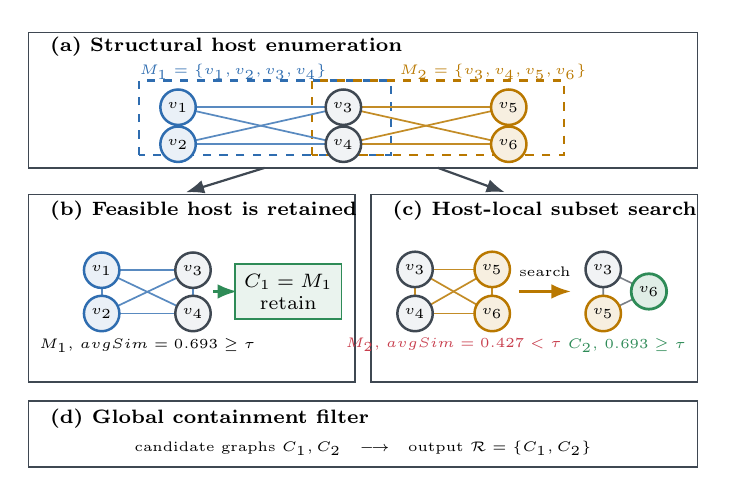
\begin{tikzpicture}[
  font=\scriptsize,
  >=Latex,
  vertex/.style={circle, draw=paperink, fill=white, line width=0.7pt,
    minimum size=4.5mm, inner sep=0pt, font=\tiny},
  mone/.style={vertex, draw=paperblue, fill=paperblue!10, line width=0.9pt},
  mtwo/.style={vertex, draw=papergold, fill=papergold!12, line width=0.9pt},
  shared/.style={vertex, draw=paperink, fill=papergray, line width=0.9pt},
  accepted/.style={vertex, draw=papergreen, fill=papergreen!15, line width=1.0pt},
  failed/.style={vertex, draw=paperred, fill=paperred!10, line width=1.0pt},
  edge/.style={draw=paperink!70, line width=0.58pt},
  edgeone/.style={draw=paperblue!80, line width=0.62pt},
  edgetwo/.style={draw=papergold!85, line width=0.62pt},
  branch/.style={->, draw=paperink, line width=0.8pt},
  acceptarrow/.style={->, draw=papergreen, line width=0.9pt},
  searcharrow/.style={->, draw=papergold, line width=0.9pt},
  paneltitle/.style={font=\scriptsize\bfseries, anchor=west},
  note/.style={font=\tiny, align=center},
  output/.style={draw=papergreen, fill=papergreen!10, line width=0.6pt,
    minimum width=13mm, minimum height=7mm, align=center},
  reject/.style={draw=paperred, fill=paperred!8, line width=0.6pt,
    minimum width=27mm, minimum height=7mm, align=center}
]

% Structural layer: two overlapping maximal cliques are generated first.
\draw[paperink, line width=0.55pt] (-0.05,-1.02) rectangle (8.45,0.70);
\node[paneltitle] at (0.10,0.52)
  {(a) Structural host enumeration};
\node[note, text=paperblue] at (2.55,0.20) {$M_1=\{v_1,v_2,v_3,v_4\}$};
\node[note, text=papergold] at (5.85,0.20) {$M_2=\{v_3,v_4,v_5,v_6\}$};

% Host outlines are drawn before edges and vertices so their overlap is visible.
\draw[paperblue, dashed, line width=0.8pt] (1.35,-0.86) rectangle (4.55,0.09);
\draw[papergold, dashed, line width=0.8pt] (3.55,-0.86) rectangle (6.75,0.09);
\begin{scope}
  \coordinate (v1) at (1.85,-0.25);
  \coordinate (v2) at (1.85,-0.72);
  \coordinate (v3) at (3.95,-0.25);
  \coordinate (v4) at (3.95,-0.72);
  \coordinate (v5) at (6.05,-0.25);
  \coordinate (v6) at (6.05,-0.72);
  \foreach \a/\b in {v1/v2,v1/v3,v1/v4,v2/v3,v2/v4,v3/v4}
    {\draw[edgeone] (\a)--(\b);}
  \foreach \a/\b in {v3/v4,v3/v5,v3/v6,v4/v5,v4/v6,v5/v6}
    {\draw[edgetwo] (\a)--(\b);}
  \node[mone] at (v1) {$v_1$};
  \node[mone] at (v2) {$v_2$};
  \node[shared] at (v3) {$v_3$};
  \node[shared] at (v4) {$v_4$};
  \node[mtwo] at (v5) {$v_5$};
  \node[mtwo] at (v6) {$v_6$};
\end{scope}

% The two hosts enter independent semantic processing branches.
\draw[branch] (2.95,-1.02)--(1.95,-1.33);
\draw[branch] (5.15,-1.02)--(6.00,-1.33);

% Feasible host: no subset search is needed.
\draw[paperink, line width=0.55pt] (-0.05,-3.74) rectangle (4.10,-1.36);
\node[paneltitle] at (0.10,-1.57) {(b) Feasible host is retained};
\begin{scope}
  \coordinate (a) at (0.88,-2.32);
  \coordinate (b) at (0.88,-2.87);
  \coordinate (c) at (2.04,-2.32);
  \coordinate (d) at (2.04,-2.87);
  \foreach \x/\y in {a/b,a/c,a/d,b/c,b/d,c/d} {\draw[edgeone] (\x)--(\y);}
  \node[mone] at (a) {$v_1$};
  \node[mone] at (b) {$v_2$};
  \node[shared] at (c) {$v_3$};
  \node[shared] at (d) {$v_4$};
\end{scope}
\node[note] at (1.46,-3.28) {$M_1$, $\operatorname{avgSim}=0.693\geq\tau$};
\draw[acceptarrow] (2.30,-2.59)--(2.60,-2.59);
\node[output] at (3.25,-2.59) {$C_1=M_1$\\retain};

% Infeasible host: bounded subset search recovers a semantic clique.
\draw[paperink, line width=0.55pt] (4.30,-3.74) rectangle (8.45,-1.36);
\node[paneltitle] at (4.45,-1.57) {(c) Host-local subset search};
\begin{scope}
  \coordinate (a) at (4.86,-2.31);
  \coordinate (b) at (4.86,-2.87);
  \coordinate (c) at (5.84,-2.31);
  \coordinate (d) at (5.84,-2.87);
  \foreach \x/\y in {a/b,a/c,a/d,b/c,b/d,c/d} {\draw[edgetwo] (\x)--(\y);}
  \node[shared] at (a) {$v_3$};
  \node[shared] at (b) {$v_4$};
  \node[mtwo] at (c) {$v_5$};
  \node[mtwo] at (d) {$v_6$};
\end{scope}
\node[note, text=paperred] at (5.35,-3.27) {$M_2$, $\operatorname{avgSim}=0.427<\tau$};
\draw[searcharrow] (6.18,-2.59)--(6.84,-2.59)
  node[midway,above=0.55mm,note] {search};
\begin{scope}
  \coordinate (a) at (7.25,-2.31);
  \coordinate (b) at (7.25,-2.87);
  \coordinate (c) at (7.83,-2.59);
  \draw[edge] (a)--(b)--(c)--cycle;
  \node[shared] at (a) {$v_3$};
  \node[mtwo] at (b) {$v_5$};
  \node[accepted] at (c) {$v_6$};
\end{scope}
\node[note, text=papergreen] at (7.55,-3.28) {$C_2$, $0.693\geq\tau$};

% Global containment removes duplicates and emits the surviving outputs.
\draw[paperink, line width=0.55pt] (-0.05,-4.82) rectangle (8.45,-3.98);
\node[paneltitle] at (0.10,-4.20) {(d) Global containment filter};
\node[note] at (4.20,-4.58)
  {candidate graphs $C_1,C_2$ \; $\longrightarrow$ \; output $\mathcal{R}=\{C_1,C_2\}$};
\end{tikzpicture}
\end{document}
